\documentclass[10pt,twoside,letterpaper]{phstylee}
\usepackage{lmodern}
\usepackage{amssymb,amsmath}
\usepackage{ifxetex,ifluatex}
\usepackage{fixltx2e} % provides \textsubscript
\ifnum 0\ifxetex 1\fi\ifluatex 1\fi=0 % if pdftex
  \usepackage[T1]{fontenc}
  \usepackage[utf8]{inputenc}
\else % if luatex or xelatex
  \ifxetex
    \usepackage{mathspec}
  \else
    \usepackage{fontspec}
  \fi
  \defaultfontfeatures{Ligatures=TeX,Scale=MatchLowercase}
\fi
% use upquote if available, for straight quotes in verbatim environments
\IfFileExists{upquote.sty}{\usepackage{upquote}}{}
% use microtype if available
\IfFileExists{microtype.sty}{%
\usepackage{microtype}
\UseMicrotypeSet[protrusion]{basicmath} % disable protrusion for tt fonts
}{}
\usepackage[bookmarks=true,bookmarksnumbered,colorlinks=true,linkcolor=black,citecolor=black,pdfstartview=FitH,linktocpage]{hyperref}
\hypersetup{unicode=true,
            pdfauthor={ALFONSO ANDRÉS TOBAR ARANCIBIA},
            pdfborder={0 0 0},
            breaklinks=true}
\urlstyle{same}  % don't use monospace font for urls
\usepackage{natbib}
\bibliographystyle{apalike}
\usepackage{color}
\usepackage{fancyvrb}
\newcommand{\VerbBar}{|}
\newcommand{\VERB}{\Verb[commandchars=\\\{\}]}
\DefineVerbatimEnvironment{Highlighting}{Verbatim}{commandchars=\\\{\}}
% Add ',fontsize=\small' for more characters per line
\usepackage{framed}
\definecolor{shadecolor}{RGB}{248,248,248}
\newenvironment{Shaded}{\begin{snugshade}}{\end{snugshade}}
\newcommand{\AlertTok}[1]{\textcolor[rgb]{0.94,0.16,0.16}{#1}}
\newcommand{\AnnotationTok}[1]{\textcolor[rgb]{0.56,0.35,0.01}{\textbf{\textit{#1}}}}
\newcommand{\AttributeTok}[1]{\textcolor[rgb]{0.77,0.63,0.00}{#1}}
\newcommand{\BaseNTok}[1]{\textcolor[rgb]{0.00,0.00,0.81}{#1}}
\newcommand{\BuiltInTok}[1]{#1}
\newcommand{\CharTok}[1]{\textcolor[rgb]{0.31,0.60,0.02}{#1}}
\newcommand{\CommentTok}[1]{\textcolor[rgb]{0.56,0.35,0.01}{\textit{#1}}}
\newcommand{\CommentVarTok}[1]{\textcolor[rgb]{0.56,0.35,0.01}{\textbf{\textit{#1}}}}
\newcommand{\ConstantTok}[1]{\textcolor[rgb]{0.00,0.00,0.00}{#1}}
\newcommand{\ControlFlowTok}[1]{\textcolor[rgb]{0.13,0.29,0.53}{\textbf{#1}}}
\newcommand{\DataTypeTok}[1]{\textcolor[rgb]{0.13,0.29,0.53}{#1}}
\newcommand{\DecValTok}[1]{\textcolor[rgb]{0.00,0.00,0.81}{#1}}
\newcommand{\DocumentationTok}[1]{\textcolor[rgb]{0.56,0.35,0.01}{\textbf{\textit{#1}}}}
\newcommand{\ErrorTok}[1]{\textcolor[rgb]{0.64,0.00,0.00}{\textbf{#1}}}
\newcommand{\ExtensionTok}[1]{#1}
\newcommand{\FloatTok}[1]{\textcolor[rgb]{0.00,0.00,0.81}{#1}}
\newcommand{\FunctionTok}[1]{\textcolor[rgb]{0.00,0.00,0.00}{#1}}
\newcommand{\ImportTok}[1]{#1}
\newcommand{\InformationTok}[1]{\textcolor[rgb]{0.56,0.35,0.01}{\textbf{\textit{#1}}}}
\newcommand{\KeywordTok}[1]{\textcolor[rgb]{0.13,0.29,0.53}{\textbf{#1}}}
\newcommand{\NormalTok}[1]{#1}
\newcommand{\OperatorTok}[1]{\textcolor[rgb]{0.81,0.36,0.00}{\textbf{#1}}}
\newcommand{\OtherTok}[1]{\textcolor[rgb]{0.56,0.35,0.01}{#1}}
\newcommand{\PreprocessorTok}[1]{\textcolor[rgb]{0.56,0.35,0.01}{\textit{#1}}}
\newcommand{\RegionMarkerTok}[1]{#1}
\newcommand{\SpecialCharTok}[1]{\textcolor[rgb]{0.00,0.00,0.00}{#1}}
\newcommand{\SpecialStringTok}[1]{\textcolor[rgb]{0.31,0.60,0.02}{#1}}
\newcommand{\StringTok}[1]{\textcolor[rgb]{0.31,0.60,0.02}{#1}}
\newcommand{\VariableTok}[1]{\textcolor[rgb]{0.00,0.00,0.00}{#1}}
\newcommand{\VerbatimStringTok}[1]{\textcolor[rgb]{0.31,0.60,0.02}{#1}}
\newcommand{\WarningTok}[1]{\textcolor[rgb]{0.56,0.35,0.01}{\textbf{\textit{#1}}}}
\usepackage{longtable,booktabs}
\IfFileExists{parskip.sty}{%
\usepackage{parskip}
}{% else
\setlength{\parindent}{0pt}
\setlength{\parskip}{6pt plus 2pt minus 1pt}
}
\setlength{\emergencystretch}{3em}  % prevent overfull lines
\providecommand{\tightlist}{%
  \setlength{\itemsep}{0pt}\setlength{\parskip}{0pt}}
\setcounter{secnumdepth}{5}
% Redefines (sub)paragraphs to behave more like sections
\ifx\paragraph\undefined\else
\let\oldparagraph\paragraph
\renewcommand{\paragraph}[1]{\oldparagraph{#1}\mbox{}}
\fi
\ifx\subparagraph\undefined\else
\let\oldsubparagraph\subparagraph
\renewcommand{\subparagraph}[1]{\oldsubparagraph{#1}\mbox{}}
\fi

%%% Use protect on footnotes to avoid problems with footnotes in titles
\let\rmarkdownfootnote\footnote%
\def\footnote{\protect\rmarkdownfootnote}






\usepackage[spanish]{varioref}%round]{natbib} %ARREGLAR varioref
\usepackage[spanish]{babel}
%\usepackage{amsfonts}
%\usepackage{amssymb}
%\usepackage{amsxtra}

\usepackage{epsfig}
\usepackage{graphicx}
\usepackage{enumerate}
\usepackage{float}
\usepackage{indentfirst}
\usepackage{graphicx}
\usepackage{rotating}
\usepackage{verbatim}
\usepackage{setspace}
%\usepackage{cite}
%\usepackage[sort&compress]{natbib}
\usepackage{color}
\usepackage{makeidx}
\addto{\captionsspanish}{\renewcommand{\bibname}{REFERENCIAS}}

%==================
%CORTES DE PALABRAS
%==================

\hyphenation{di-men-sio-na-das glo-ba-les an-te-rior-men-te res-prec-to des-cri-tas con-ti-nua-cion cons-truc-cion ad-mi-si-ble
ho-ri-zon-ta-les
con-si-de-ra-ble res-trin-gi-da pro-ce-di-mien-to pro-ce-di-mien-tos
pro-ble-ma con-ti-nua-cion ad-mi-si-bles sen-si-bi-li-dad
es-ta-bi-li-dad pa-ra-me-tri-za-cion co-ro-la-rio fun-cio-nal
per-te-ne-cen fac-to-ri-za-cio-nes trans-fe-ren-cia rea-li-zar
co-pri-mas iz-quier-das ob-te-ne-mos pa-ra res-trin-gi-do u-san-do
mo-di-fi-ca-do des-pren-den cons-ti-tu-ye pro-ba-bi-li-dad
pro-ba-bi-li-da-des res-pues-ta va-lor ge-ne-ra-cion o-ri-gi-na-les
a-su-mien-do con-si-de-ra-das a-pro-xi-ma-cion res-tric-cio-nes
e-le-men-to va-ria-ble su-per-in-di-ce in-de-pen-dien-te e-di-fi-cio
des-pla-za-mien-to re-fe-ren-cia si-guien-te res-tric-cion
dis-po-si-ti-vos ni-vel res-tric-ti-vas e-le-men-tos ho-ri-zon-tal
va-ria-bles cons-tan-te cons-tan-tes con-fia-bi-li-dad res-tric-cion
fa-lla fa-llas gra-dien-te res-pe-tar so-li-ci-ta-cion p-ci-rren-tes}

\begin{document}


%
% Tapa

\pagestyle{empty}

\begin{center}

\begin{center}
  
\includegraphics{images/logo_new.png}
\end{center}


\large \textbf{UNIVERSIDAD TÉCNICA FEDERICO SANTA MARÍA}

\large \textbf{DEPARTAMENTO DE OBRAS CIVILES}

\vspace{40mm}

\Large {\bf USO DE REDES CONVOLUCIONALES PARA LA ESTMACIÓN DE LA INCERTIDUMBRE MEDIANTE CAMPOS ALEATORIOS}

\vspace{40mm}

\large \textbf{ALFONSO ANDRÉS TOBAR ARANCIBIA}

\vspace{5mm}

\textbf{Ingeniero Civil}\\




\vspace{5mm}
Junio de 2020


\end{center}

% FIN TAPA

% PORTADA

\pagestyle{empty}

\begin{center}

\begin{center}
  
\includegraphics{images/logo_new.png}
\end{center}


\large \textbf{UNIVERSIDAD TÉCNICA FEDERICO SANTA MARÍA}

\large \textbf{DEPARTAMENTO DE OBRAS CIVILES}

\vspace{20mm}

\Large {\bf USO DE REDES CONVOLUCIONALES PARA LA ESTMACIÓN DE LA INCERTIDUMBRE MEDIANTE CAMPOS ALEATORIOS}

\vspace{15mm}

\normalsize Memoria de Título presentada por

\large \textbf{ALFONSO ANDRÉS TOBAR ARANCIBIA}

\vspace{15mm}

\normalsize Como requisito parcial para optar al título de

\textbf{Ingeniero Civil}

\vspace{2.5mm}

%y al grado de

%\textbf{Magíster en Ciencias de la Ingeniería Civil}

\vspace{15mm}

Profesor Guía

Marcos Valdebenito %Dr. Marcos Alberto Valdebenito Castillo

\vspace{5mm}
Junio de 2020


\end{center}

%\cleardoublepage

\vspace{5mm}

\noindent USO DE REDES CONVOLUCIONALES PARA LA ESTMACIÓN DE LA INCERTIDUMBRE MEDIANTE CAMPOS ALEATORIOS.

\vspace{5mm}

%TITULO %\noindent{\large {\bf DESARROLLO DE ESTRATEGIAS EFICIENTES PARA CUANTIFICAR LA INCERTEZA EN SISTEMAS ESTRUCTURALES LINEALES}}

\vspace{25mm}

\noindent AUTOR

\vspace{5mm}

\noindent{\large {\bf ALFONSO ANDRÉS TOBAR ARANCIBIA}}

\vspace{20mm}

\noindent TRABAJO DE MEMORIA, presentado en cumplimiento parcial de
los requisitos para el título de Ingeniero Civil %y el grado de
%Magíster en Ciencias de la Ingeniería Civil 
de la Universidad Técnica Federico Santa María.

\vspace{20mm}

\begin{tabular}{p{60mm}c}
COMISIÓN 
\vspace{2mm}
\\
Marcos Valdebenito & \rule{60mm}{1pt} \\
& \\
& \\
Patricio Bonelli & \rule{60mm}{1pt} \\
& \\
& \\
Ludwig Stowhas & \rule{60mm}{1pt} \\
&
\end{tabular}

\vspace{30.5mm}

\hfill Valparaíso, Chile, Junio de 2020.

\cleardoublepage

%\thispagestyle{empty}

  %\vspace{300mm}

%\begin{center}
%
\includegraphics{images_JComicheo/portada.pdf}
%\end{center}
%\begin{center}
%
\includegraphics[scale=0.23]{images_JComicheo/portada.pdf}
%\end{center}
%\begin{center}
%
\includegraphics[scale=0.23]{images_JComicheo/portada.pdf}
%\end{center}
%\begin{center}
%
\includegraphics[scale=0.23]{images_JComicheo/portada.pdf}
%\end{center}
%\begin{center}
%
\includegraphics[scale=0.23]{images_JComicheo/portada.pdf}
%\end{center}




\begin{flushright}
\large{\emph{}}
\end{flushright}
\begin{center}

\includegraphics{images/portada.pdf}
\end{center}



%
\begin{flushright}
\large{\emph{Hasta que salió}}
\end{flushright}
%
\cleardoublepage

%  FIN PORTADA

%\pagestyle{fancyplain}
\pagenumbering{roman}

\chapter*{AGRADECIMIENTOS}
The preface pretty much says it all.

Second paragraph of abstract starts here.
\cleardoublepage

\chapter*{RESUMEN}
The preface pretty much says it all.

Second paragraph of abstract starts here.
\cleardoublepage

\chapter*{ABSTRACT}
The preface pretty much says it all.

Second paragraph of abstract starts here.
\cleardoublepage




{
\setcounter{tocdepth}{1}
\phantomsection
\addcontentsline{toc}{chapter}{CONTENIDO}
\renewcommand\contentsname{CONTENIDO}
\tableofcontents
}

\renewcommand\listfigurename{ÍNDICE DE FIGURAS}
\listoffigures
\cleardoublepage

\renewcommand\listtablename{ÍNDICE DE TABLAS}
\listoftables
\cleardoublepage

\pagenumbering{arabic}
\pagestyle{fancy}

\hypertarget{prerequisites}{%
\chapter*{Prerequisites}\label{prerequisites}}
\addcontentsline{toc}{chapter}{Prerequisites}

This is a \emph{sample} book written in \textbf{Markdown}. You can use anything that Pandoc's Markdown supports, e.g., a math equation \(a^2 + b^2 = c^2\).

The \textbf{bookdown} package can be installed from CRAN or Github:

\begin{Shaded}
\begin{Highlighting}[]
\KeywordTok{install.packages}\NormalTok{(}\StringTok{"bookdown"}\NormalTok{)}
\CommentTok{# or the development version}
\CommentTok{# devtools::install_github("rstudio/bookdown")}
\end{Highlighting}
\end{Shaded}

Remember each Rmd file contains one and only one chapter, and a chapter is defined by the first-level heading \texttt{\#}.

To compile this example to PDF, you need XeLaTeX. You are recommended to install TinyTeX (which includes XeLaTeX): \url{https://yihui.name/tinytex/}.

\hypertarget{intro}{%
\chapter{Introduction}\label{intro}}

You can label chapter and section titles using \texttt{\{\#label\}} after them, e.g., we can reference Chapter \ref{intro}. If you do not manually label them, there will be automatic labels anyway, e.g., Chapter \ref{methods}.

Figures and tables with captions will be placed in \texttt{figure} and \texttt{table} environments, respectively.

\begin{Shaded}
\begin{Highlighting}[]
\KeywordTok{par}\NormalTok{(}\DataTypeTok{mar =} \KeywordTok{c}\NormalTok{(}\DecValTok{4}\NormalTok{, }\DecValTok{4}\NormalTok{, }\FloatTok{.1}\NormalTok{, }\FloatTok{.1}\NormalTok{))}
\KeywordTok{plot}\NormalTok{(pressure, }\DataTypeTok{type =} \StringTok{'b'}\NormalTok{, }\DataTypeTok{pch =} \DecValTok{19}\NormalTok{)}
\end{Highlighting}
\end{Shaded}

\begin{figure}

{\centering 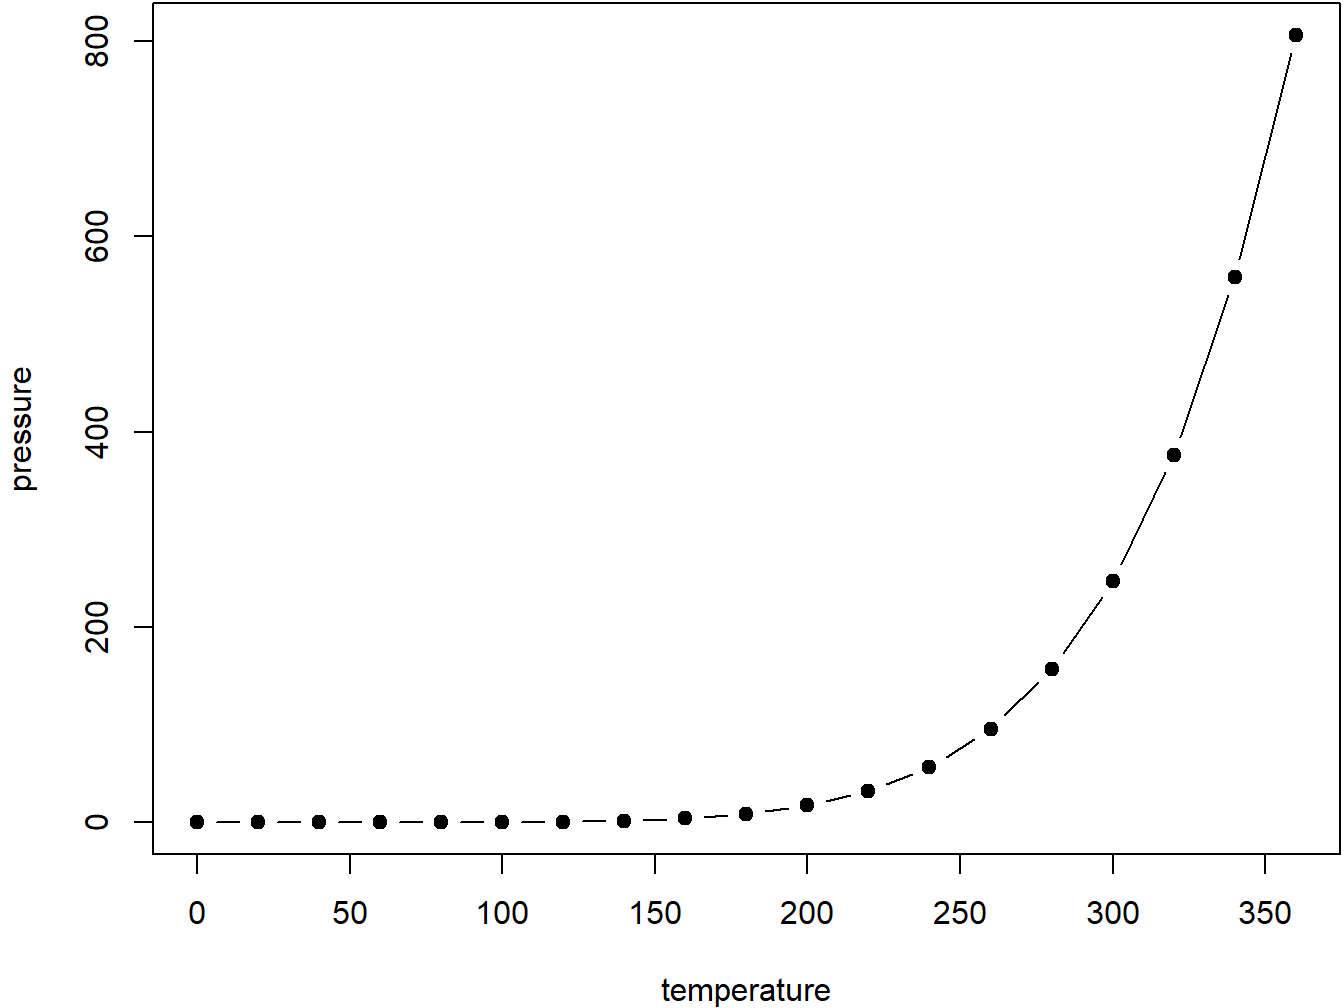
\includegraphics[width=0.8\linewidth]{Tesis_files/figure-latex/nice-fig-1} 

}

\caption{Here is a nice figure!}\label{fig:nice-fig}
\end{figure}

Reference a figure by its code chunk label with the \texttt{fig:} prefix, e.g., see Figure \ref{fig:nice-fig}. Similarly, you can reference tables generated from \texttt{knitr::kable()}, e.g., see Table \ref{tab:nice-tab}.

\begin{Shaded}
\begin{Highlighting}[]
\NormalTok{knitr}\OperatorTok{::}\KeywordTok{kable}\NormalTok{(}
  \KeywordTok{head}\NormalTok{(iris, }\DecValTok{20}\NormalTok{), }\DataTypeTok{caption =} \StringTok{'Here is a nice table!'}\NormalTok{,}
  \DataTypeTok{booktabs =} \OtherTok{TRUE}
\NormalTok{)}
\end{Highlighting}
\end{Shaded}

\begin{table}

\caption{\label{tab:nice-tab}Here is a nice table!}
\centering
\begin{tabular}[t]{rrrrl}
\toprule
Sepal.Length & Sepal.Width & Petal.Length & Petal.Width & Species\\
\midrule
5.1 & 3.5 & 1.4 & 0.2 & setosa\\
4.9 & 3.0 & 1.4 & 0.2 & setosa\\
4.7 & 3.2 & 1.3 & 0.2 & setosa\\
4.6 & 3.1 & 1.5 & 0.2 & setosa\\
5.0 & 3.6 & 1.4 & 0.2 & setosa\\
\addlinespace
5.4 & 3.9 & 1.7 & 0.4 & setosa\\
4.6 & 3.4 & 1.4 & 0.3 & setosa\\
5.0 & 3.4 & 1.5 & 0.2 & setosa\\
4.4 & 2.9 & 1.4 & 0.2 & setosa\\
4.9 & 3.1 & 1.5 & 0.1 & setosa\\
\addlinespace
5.4 & 3.7 & 1.5 & 0.2 & setosa\\
4.8 & 3.4 & 1.6 & 0.2 & setosa\\
4.8 & 3.0 & 1.4 & 0.1 & setosa\\
4.3 & 3.0 & 1.1 & 0.1 & setosa\\
5.8 & 4.0 & 1.2 & 0.2 & setosa\\
\addlinespace
5.7 & 4.4 & 1.5 & 0.4 & setosa\\
5.4 & 3.9 & 1.3 & 0.4 & setosa\\
5.1 & 3.5 & 1.4 & 0.3 & setosa\\
5.7 & 3.8 & 1.7 & 0.3 & setosa\\
5.1 & 3.8 & 1.5 & 0.3 & setosa\\
\bottomrule
\end{tabular}
\end{table}

You can write citations, too. For example, we are using the \textbf{bookdown} package \citep{R-bookdown} in this sample book, which was built on top of R Markdown and \textbf{knitr} \citep{xie2015}.

\hypertarget{literature}{%
\chapter{Literature}\label{literature}}

Here is a review of existing methods.

\hypertarget{methods}{%
\chapter{Methods}\label{methods}}

We describe our methods in this chapter.

\hypertarget{applications}{%
\chapter{Applications}\label{applications}}

Some \emph{significant} applications are demonstrated in this chapter.

\hypertarget{example-one}{%
\section{Example one}\label{example-one}}

\hypertarget{example-two}{%
\section{Example two}\label{example-two}}

\hypertarget{final-words}{%
\chapter{Final Words}\label{final-words}}

We have finished a nice book.

\bibliography{book.bib,packages.bib}


\end{document}
